\documentclass[12pt,a4paper]{article}

\usepackage[T1]{fontenc}
\usepackage[english]{babel}
\usepackage[utf8]{inputenc}
\usepackage{lmodern}
\usepackage{caption}
\usepackage{braket}
\usepackage{float}
\usepackage{hyperref}
\usepackage{algorithm}
\usepackage{algpseudocode}
\usepackage{amssymb}
\usepackage{graphicx}
\usepackage[backend=biber,style=numeric,maxnames=5]{biblatex}
\usepackage{csquotes}
\usepackage{amsmath}
\addbibresource{comparison.bib}

\begin{document}


\begin{center}\large\textbf{QKD comparison}\end{center}
\hspace{7cm}
\section{Introduction}
Tl;dr most of experiments use modified bb84 with the biggest difference of encoding states during the exchange to increase the key rate and decrease the loss/error rate. The second part around DI-QKD uses qkd based on E91 or different variations of the CHSH game. 
\subsection{Types of QKD}
We can divide qkd into 4 main types \cite{sobinskagroup}
\begin{itemize}
    \item Prepare and measure QKD
    \item Measurement-Device-Independent QKD
    \item Entanglement based QKD
    \item Device independent QKD
\end{itemize}
\begin{figure}[h]
    \centering
    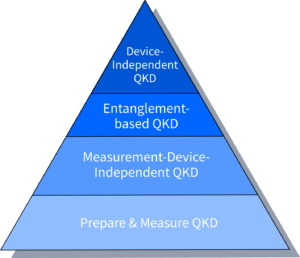
\includegraphics[width=0.5\textwidth]{media/image.png}
    \caption{Source: \cite{klucz_zrodlowy}}
    \label{fig:moj_obrazek}
\end{figure}
Prepare and measure QKD  to BB84 and BB92 Sarg04\cite{bennett1984quantum} \cite{bennett1992quantum} possible various attacks: commonly discussed are trojan horse attack and photon number splitting \cite{lo2014secure}, \cite{xu2020secure} 

BB84 security is dependent on two conditions, no-cloning theorem and existence of an authenticated classical channel of communication for Alice and Bob.

Entanglement-based QKD to E91 \cite{ekert1991quantum}
Entanglement based protocols use properties of correlation for entanglement qubits.

Device-independent QKD is the highest level security class, those protocols can be safely implemented with untrusted/unknown devices.  
\cite{primaatmaja2020security}, E91 wasn't created as DI-QKD, but is also based on CHSH games\cite{zapatero2023advances}
\\ entaglement-based QKDs are worse on implementation than, prepare and measure. \\ DI-QKD is mostly oriented around devices and their limitations; therefore, we could focus only on Entaglement-based and Prepare  \& measure QKD \\
\url{https://doi.org/10.1103/PhysRevA.78.020301} The
security of entanglement-based implementations can be
based on the sole knowledge of the error rate, because this
quantity already contains information about the imperfection
of the source, while such imperfections, for example, the photonnumber statistics or spectral distinguishability of different letters, must be carefully taken into account in preparation and measurement schemes. \url{https://journals.aps.org/prl/abstract/10.1103/PhysRevLett.90.057902}
\section{Protocols and implementations}
\begin{figure}[H]
    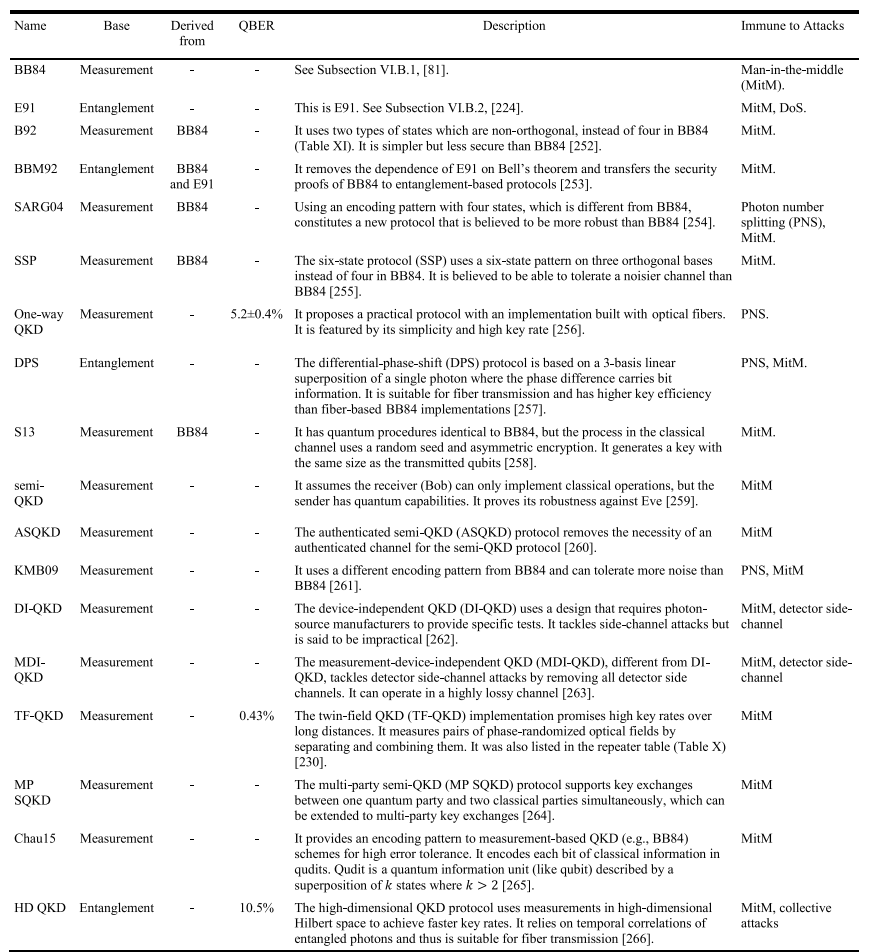
\includegraphics[width=1\textwidth]{media/Screenshot 2025-07-07 133153.png}
    \caption{Source: \cite{ieee_qkd_overview_2023}}
\end{figure}
\begin{figure}[H]
    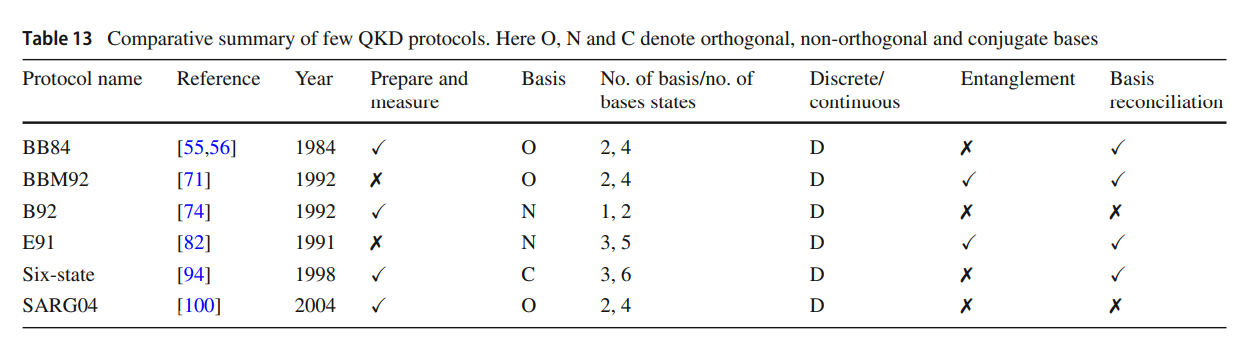
\includegraphics[width=1\textwidth]{media/Screenshot 2025-07-07 191015.png}
    \caption{Source: \cite{springer_qkd_chapter_2017}}
\end{figure}
\section{QKD testing}
Numerical calculations of the finite key rate:
\url{https://journals.aps.org/prresearch/abstract/10.1103/PhysRevResearch.3.013274}
\\

\section{Comparison}
The biggest difference between known QKDs is the asymmetrical approach of QKD based on discrimination (QKD-D). In most of used QKDs quantum states prepared by Alice and Bob are the same and have the same dimensional space, and also sets of used measurements are the same for A and B. In QKD-D both parties have different sets of von Neumann measurements: $(\mathcal{Q}_i)_{i=0,\dots,d-1}$ for Bob and $\mathcal{P}_d$ for Alice where d denotes the number of dimensions in the quantum state used by them. 
\\Similarly to BB84 the idea of the protocol is that we cannot cannot perfectly distinguish between non-orthogonal quantum states, both protocol are prepare \& measure and do not need to use an entanglement to perform and validate measurements. Both QKD should have similar vulnerabilities and possible attacks? [expand] \\ 
BB84 security is based on the no-clone theorem. The detection of eavesdropper is just by checking post-selected outcomes when selected bases were the same. This approach reduces by 50\% the number of bits used to create a key. \\
E91 uses a different technique; the security is based on Bell's theorem and is calculating $E(\theta_A, \theta_B) = -\cos(\theta_A - \theta_B)$ to detect eavesdropping. The angles used are specifically used to detect quantum correlations, so there is a need to use entanglement states (in E91 the Bell's state is proposed to reduce complexity of the task $|\psi^-\rangle = \frac{1}{\sqrt{2}} (|01\rangle - |10\rangle)$ verify?). This approach initially reduces the number of usable bits, but thanks to this we can use bits when the bases do not match to perform the eve detection, which means we have a higher percentage of bits actually used to generate the key. \\
The QKD-D approach does not need to use entanglement to check the security of the transmission with the use of outcomes for different bases. Validation is performed by checking if the discrimination of von Neumann measurements was optimal if not the security of protocol is compromised?

\begin{table}[h!]
  \centering
  \begin{tabular}{|l|l|l|l|}
    \hline
     &BB84 & E91 &  QKD-D \\
    \hline
    No. Dimensions & $\mathbb{C}^2$ & $\mathbb{C}^2$ & $\mathbb{C}^2$ or $\mathbb{C}^4$ \\
    \hline
    Measurement bases &	Z basis and X basis&  Axes on Bloch sphere &  $\mathcal{P}_d$ and  $\mathcal{Q}_d$ POVMs \\
    \hline
    A and B actions & Symmetrical &  Symmetrical &  Asymmetrical \\
    \hline
        Security based on &	No clone theorem&  Bell's theorem &  Optimal discrimination \\
    \hline
    Eve detection&	Postselection& CHSH inequality &  Discimination \\
    \hline
  \end{tabular}
\end{table}

\section{BB84}
\url{https://doi.org/10.1016/j.tcs.2014.05.025}
\begin{algorithm}
\caption{BB84 protocol}
\begin{algorithmic}[1]
\State Alice chooses $n$ random bits by flipping a coin.
\State Alice again flip coin n-times for determining the basis used for each corresponding random bit.
\State Alice prepares the random bits in their corresponding basis and sends to Bob.
\State Bob does not know the basis corresponding to each random bit. He tosses the coin n-times. He measures the received qubit in the obtained random basis after tossing the coin. Bob announces the receipt of states.
\State Alice and Bob publicly compare their bases using an authentic classical channel. Alice informs the Bob regarding bases agreement and disagreement. If they disagree on a particular basis, they drop the corresponding bit. Now Bob will get only n/2 random bits and n/2 random bits are scratch out.
\State Bob randomly choose half of the remaining n/2 random bits
obtained from Step 5 and compare with Alice publicly. If both disagree above a permitted allowed errors (due to noise), then they drop the complete sequence of random bits and it indicate that Eve was listening. If these n/4 random bits are almost similar (i.e. within permitted allowed error due to noise) means Eve was not listening. In this case, remaining n/4 will be used as a random key between Alice and Bob.
\State Algorithm \url{https://link.springer.com/article/10.1007/s11831-021-09561-2}
\end{algorithmic}
\end{algorithm}
BB84 uses 4 stateS:
$\ket{1}, \ket{0}, \ket{+}, \ket{-}$
Alice send random stream of qubits to Bob and he measures them in standard or Hadamard basis
Eve is detected when QBER is at least 25\%

\section{Photon Number splitting attack}
Weak coherent pulses were used in prepare \& measure QKD but weak states are vulnerable to the photon number splitting attack (PNS). 
There were two major proposes to mitigate such problem, by using Sarg04 and decoy-state method. Sarg04 is using different postselection to reduce the effect of PNS attack, but the advantage of maintaining experimental machinery intact is reduced by only half of efficiency for key rate in commparison with BB84

Decoy State, DPS, COW

Entaglement based QKD and CV-QKD


Using flaws in the devices, sender is not sending one photon but a beam of photons \href{https://link.springer.com/chapter/10.1007/978-3-319-56246-9_12}{The projection into these subspaces does not modify the polarization of the
photons. Then she performs a polarization-preserving splitting operation, for
example, by an interaction described by a Jaynes-Cummings Hamiltonian or an
active arrangement of beam-splitters combined with further QND measurements.
She keeps one photon and sends the other (n-1) photons to Bob.}
\section{Decoy State}
It is an additional layer of security for QKDs, lowering the real-life key rate. \\
The decoy-state method is a common way to combat source
imperfection by introducing additional sources for better channel
characterization. In the decoy-state method, the user randomly
modifies the source states during the quantum stage; after
that, he or she reveals which state is used in each turn. Eve
cannot modify her attack to different source states, but in
post-processing the users can estimate their parameters conditioned on that knowledge. The decoy-state method is used
mostly to bound the multiphoton components in a practical
photon source. \\
Instead of sending signals of equal intensity, Alice first chooses the intensity of each signal at random from a set of prescribed values. States sent
with one particular intensity are called signal states, whereas states
sent with other intensities are called decoy states. Once Bob has
detected all the signals, Alice broadcasts the intensity used for
each pulse
\url{https://www.nature.com/articles/nphoton.2014.149}
\section{SARG04}
\url{https://doi.org/10.1103/PhysRevLett.92.057901}
Used to solve PNS when using weak laser pulses
Encoding the classical bit into pairs of non-orthogonal states.
Instead of revealing the basis Alice publicly announces one of the four pairs of states. Bob can deduce which state was sent depending on his measurement and sent pair. It makes post-selection more complicated but still uses BB84 protocol
If measurement result is orthogonal to one of the states in pair the second one creates the key if not discard measurement.
Key rate same to BB84 1/4
\url{https://arxiv.org/pdf/quant-ph/0510025} Hee for two way communication bit rate toleration 19,4\% for one photon source, 6,5\% to photon source
\url{https://arxiv.org/pdf/quant-ph/0505035}
\section{Three state protocol}
\url{https://journals.aps.org/prl/abstract/10.1103/PhysRevLett.85.3313}
\section{Six-State protocol SSP}
\url{https://doi.org/10.1103/PhysRevLett.81.3018}
Generalization of BB84 using 3 conjugate base -> six states \\More secure because there are more states. but losing 2/3 of signal (in bb84 it is only 1/2)
\section{E91}
\url{https://doi.org/10.1103/PhysRevLett.67.661}
In \cite{ekert1991quantum} used
\begin{align*}
Alice: \\
\phi_1^a &= 0 \\
\phi_2^a &= \frac{\pi}{4} \\
\phi_3^a &= \frac{\pi}{2} \\
Bob: \\
\phi_1^b &= \frac{\pi}{4} \\
\phi_2^b &= \frac{\pi}{2} \\
\phi_3^b &= \frac{3\pi}{4}
\end{align*}
If same orientation, outcome creates a key, if not perform perform test to check if eve
1/3 transmission used to generate a key, 2/3 to check if no eavesdropper \\
\href{https://journals.sagepub.com/doi/full/10.1177/1550147718778192} {Modified E91} \\ 
\url{https://arxiv.org/pdf/2212.13837} here in the direct photon allocation 25\% is used to generate key, 50\% to validate, 25\% discarded.
\section{B92}
The simplified version of BB84 uses only two states $\ket{0}, \ket{+}$ In B92 Bob does not announce the basis he used. States: $\ket{1}, \ket{-}$ are only kept to create bit string. 1/4 of usable bits
\url{https://doi.org/10.1103/PhysRevLett.68.3121}
Uses only two non orthogonal states, each one coding for one bit value.
However, a positive operator-valued measure (POVM) can be performed to unambiguously discriminate nonorthogonal states in most of the instances, which when executed by Eve can threaten the security of B92. 
\url{https://theses.cz/id/aa00qc/Mgr_thesis_Fadrny_20_06_07.pdf}
\section{BBM92}
\url{https://doi.org/10.1103/PhysRevLett.68.557}
Entaglement version ob BB84 without using Bell's theorem (instead, of sending from Alice to Bob, we have a central source of photons). \\
Z and X basis used to prepare the particles, and the key created where Alice and Bob selected the same basis
\section{MSZ96}
\url{https://doi.org/10.1016/0030-4018(95)00688-5}
Protocol without using polarized photons\\
Four non-orthogonal quantum states \\ Similar to BB84 but no information about key rate
\section{S13}
\url{https://doi.org/10.48550/arXiv.1311.1582}
Identical to BB84 uses just different private reconciliation
\section{KMB09}
\url{https://doi.org/10.1088/1367-2630/11/6/063043}
Oriented specifically around long-distance communication and bit error.
Time-bin N-dimensional photon states are used to send qubits, but as in BB84 they are using two mutually unbiased bases, the eavesdropper found by calculating index transmission control error.
\section{T12}
\url{https://doi.org/10.1364/OE.21.024550}
Based on BB84 and decoy state. Theoretical efficiency of T12 is 88\% because only 11\% of detected counts are discarded not 50\% that is because the X bases is the minority basis (in bb84 X and Z bases are selected equally)
\section{DPS}
\url{https://doi.org/10.1103/PhysRevLett.89.037902}
Utilizes four nonorthogonal states.A photon split into three pulses
is sent from Alice to Bob, in which the phases of two sequential probability amplitudes are randomly modulated. Bob extracts the bit information by measuring the differential phase. \\ 
(1) When Bob's detectors click in the second or third
instances, he records the time and the detector that clicks.
(2) Bob tells Alice the time instance of the photon detection. (3) From this information and her modulation data,
Alice knows which detector clicked in Bob’s site. (4) Alice and Bob have an identical bit string, provided that the
DET1 click represents “0” and the DET2 click represents
“1.” In the above protocol, Bob only tells the time-instance
to Alice, and the bit information is not leaked to the public. \\
Stil vulnerable to PNS \\ Key creation effciency 8/3 time higher than BB84 \\ The detection of Eve is depending on Eve's strategies. \\
The speed is thanks to fiber optimization without polarization there are BB84 on phase estimation but proposed 1/4 key rate.
\section{Twin Field QKD}
Rather practical cases only
The class oof Measurement Device Independent QKD
Used in long distance scenarios without quantum reapeters \url{https://www.nature.com/articles/s41586-018-0066-6}achieves post-selected entanglement by performing single-photon interference at Charlie’s side instead of a two-photon Bell state measurement, enabling it to achieve a key rate roportional to the square root of channel transmittance (O(sqrt(n))) \url{https://arxiv.org/pdf/2408.09318v1} \\ \url{https://doi.org/10.1103/PhysRevLett.130.210801} 
Similarly to dps also use phase encoding, couldn't find more about theory around it
\section{COW}
Cow protocol qkd for fibre opticis \url{https://iopscience.iop.org/article/10.1088/1367-2630/11/7/075003/meta}
\section{Chau15}
\url{https://doi.org/10.1103/PhysRevA.92.062324}
Different form of encoding qubit to increase robustness.
\section{K-State QKD}
\url{https://arxiv.org/pdf/1802.05099} Entaglement bell state, characteristics of the protocol are the same as PBC00 protocol
\section{PBC00}
\url{https://www.tandfonline.com/doi/epdf/10.1080/09500340008244056}
\url{https://www.tandfonline.com/doi/epdf/10.1080/09500340008244056}
\section{FCS QKD}
\url{https://arxiv.org/pdf/2507.11243}
MDI QKD
\section{Phase Matching QKD}
\url{https://journals.aps.org/prx/abstract/10.1103/PhysRevX.8.031043}
\section{QKD from random seed}
\url{https://arxiv.org/abs/1311.1582}
"Zero losses" 
\section{Practical tests}
\url{https://arxiv.org/pdf/2308.01036v2}
QBER for BB84, B92, E91 \\
\section{References}
\url{https://iopscience.iop.org/article/10.1088/1367-2630/11/6/063043/pdf}
\printbibliography[heading=none] 

\end{document}
